\documentclass{standalone}
\usepackage{tikz}
\begin{document}
\begin{tikzpicture}
    \draw (0,0) -- (4,0) node[anchor=north west] {x axis};
    \draw (0,0) -- (0,4) node[anchor=south east] {y axis};
    \draw (0,0) -- (3,3) node[anchor=south  west] {z axis};
\end{tikzpicture}

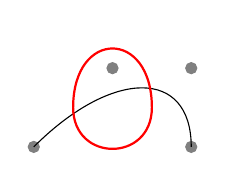
\begin{tikzpicture}
\filldraw [gray] (0,0) circle [radius=2pt]
(1,1) circle [radius=2pt]
(2,1) circle [radius=2pt]
(2,0) circle [radius=2pt];
\draw (0,0) .. controls (1,1) and (2,1) .. (2,0);
\draw[red, thick] (1.5,0.5) .. controls (1.5,1.5) and (0.5,1.5) .. (0.5,0.5)
                  .. controls (0.5,-0.2) and (1.5,-0.2) .. (1.5,0.5);
\end{tikzpicture}
\end{document}